
\subsection{Influenza della pressione}
Ragioniamo adesso su cosa succede se modifichiamo la pressione, cioè vogliamo capire se la costante di equilibrio dipende anche dalla pressione.

La pressione di ciascun componente è data dalla pressione totale per la sua frazione molare, ad esempio la pressione del componente A sarà $P_A = P_{tot} \cdot \rchi_A$\,.

Se allora abbiamo una reazione del tipo
$$\ce{\alpha A + \beta B <--> \gamma C + \delta D}$$

la costante di equilibrio potrà essere scritta come

$$k_p = \frac{P_C^{\gamma} \cdot P_D^{\delta}}{P_A^{\alpha} \cdot P_B^{\beta}} = \frac{\rchi_C^{\gamma} \cdot \rchi_D^{\delta}}{\rchi_A^{\alpha} \cdot \rchi_B^{\beta}} \cdot P_{tot}^{(\gamma + \delta - \alpha - \beta)}$$

$$\implies k_p = k_{\rchi} \cdot P^{\Delta n}$$

cioè la $k_p$ è uguale alla costante espressa in funzione delle frazioni molari per la pressione totale elevata alla variazione del numero di moli:

\begin{itemize}
    \item Se $\Delta n = 0 \implies k_p = k_{\rchi}$
    \item Se $\Delta n \neq 0 \implies k_p \neq k_{\rchi}$
\end{itemize}

\vspace{0.2cm}\textbf{ES.1}
$$\ce{H_2 + I_2 <--> 2HI}, \quad \Delta n = 0 \implies k_p = k_{\rchi}$$

\textbf{ES.2}
$$\ce{2NO + O_2 <--> 2NO_2}, \quad \Delta n = -1 \implies k_p = k_{\rchi} \cdot P^{-1}$$

$$\implies k_p = k_{\rchi} \cdot \frac{1}{P}= \frac{\rchi_{\text{NO}_2}^2}{\rchi_{\text{NO}}^2 \cdot \rchi_{\text{O}_2}} \cdot \frac{1}{P}$$

Dall'ES.2 deduciamo che $k_p$ è inversamente proporzionale alla pressione totale.

Se aumenta la pressione, affinché il rapporto resti costante dovrà aumentare il numeratore. Nel caso particolare dovrà allora aumentare la frazione molare di $\rm NO_2$.

Ne segue che se vogliamo spostare l'equilibrio verso destra, il che equivale a produrre più $\rm NO_2$ di quanto ne produce già la reazione, dobbiamo comprimere. Ciò faciliterà anche la diminuizione di volume (infatti da 3 moli di reagenti passiamo a 2 moli di prodotto) in questa specifica reazione.

\vspace{0.2cm}\textbf{ES.3 La produzione dell'ammoniaca}
$$\ce{N_2 + 3H_2 <--> 2NH_3}$$

In essa abbiamo 4 moli di reagente e due di prodotto.

La costante di equilibrio sarà

$$k_p = \frac{P_{\text{NH}_3}^2}{P_{\text{N}_2} + P_{\text{H}_2}^3}$$

In termini di frazione molare sarà

$$k_P = \frac{\rchi_{\text{NH}_3}^2}{\rchi_{\text{N}_2} + \rchi_{\text{H}_2}^3} \cdot \frac{1}{P^2}$$

Questa reazione allora sarà ancora di più influenzata dalla pressione.

\vspace{0.2cm}Quindi in una reazione non possiamo agire sulla temperatura perché cambierebbe la costante, ma fissata la temperatura possiamo variare l'equilibrio (cioè spostarlo più a destra o più a sinistra) cambiando il valore della pressione in tutte quelle reazioni laddove il numero di moli cambia con la reazione ($\Delta n \neq 0$).

\vspace{0.2cm}Va da notare che per $\Delta n > 0$, cioè se il numero di moli nei prodotti aumenta, per spostare l'equilibrio verso destra si deve abbassare la pressione.

\subsection{Influenza della temperatura}
Abbiamo detto che la temperature non puà variare, altrimenti cambia il valore della costante di equilibrio.

Consideriamo la reazione
$$\ce{N_2(g) + O_2(g) + 180.5 \, kJ/mol <--> 2NO(g)}$$

Per ottenere l'ossido di azoto dobbiamo riscaldare, cioè dobbiamo fornire calore. Abbiamo quindi immaginato che il calore sia un reagente.

Siccome questo processo richiede assorbimento di calore, cioè è un processo endotermico, si ha $\Delta$H$>0$. Aumentare calore comporterà allora un aumento del prodotto ottenuto, perché è come se aumentassimo la concentrazione dei reagenti. Il calore quindi è diventato un reagente, tant'è che la costante di equilibrio aumenta con la temperatura.

Pertanto se il calore è un reagente, l'equilibrio può essere spostato verso destra fornendo calore.

Consideriamo adesso la reazione

$$\ce{2NO_2(g) <--> N_2O_4(g) + 57.2 \, kJ/mol}$$

Il biossido di azoto ha un elettrone spaiato sull'azoto, ossia è una molecola paramagnetica. Due molecole di NO$_2$ tendono a unire questi due elettroni spaiati e formare un legame, ottenendo così il dimero (cioè una molecola formata dall'unione di due molecole uguali) N$_2$O$_4$.

In questa reazione il calore è a destra, ossia questa reazione avviene con sviluppo di calore (processo esotermico, $\Delta$H$<$0). Allora per spostare l'equilibrio verso destra dovremo raffreddare, cioè sottrarremo il calore. Infatti la costante di equilibrio di questa reazione diminuisce all'aumentare della temperatura.

Quindi se la reazione sviluppa calore, sottraiamo questo e la reazione riparte per riprodurre il calore sottratto. In altre parole tutte le volte che c'è una reazione all'equilibrio e l'equilibrio viene turbato, esso si sposta da solo per tentare di ripristinare un nuovo stato di equilibrio.

Se invece la reazione necessita riscaldamento, riscaldando la reazione ripartirà.

In questo modo sarà come aumentare, rispettivamente, le concentrazioni dei prodotti e dei reagenti.

Sostanzialmente

\begin{itemize}
    \item L'aumento di T provoca l'aumento di $k_c$ se $\Delta$H$>$0 (endotermico)
    \item L'aumento di T provoca la diminuizione di $k_c$ se $\Delta$H$<$0 (esotermico)
\end{itemize}

Torniamo all'ultima reazione.

NO$_2$ è una molecola paramagnetica perché ha un elettrone spaiato, mentre la molecola N$_2$O$_4$ non lo ha, quindi non è paramagnetica. L'elettrone spaiato fornisce un colore bruno all'NO$_2$, mentre N$_2$O$_4$ è incolore.

\begin{figure}[htp]
    \centering
    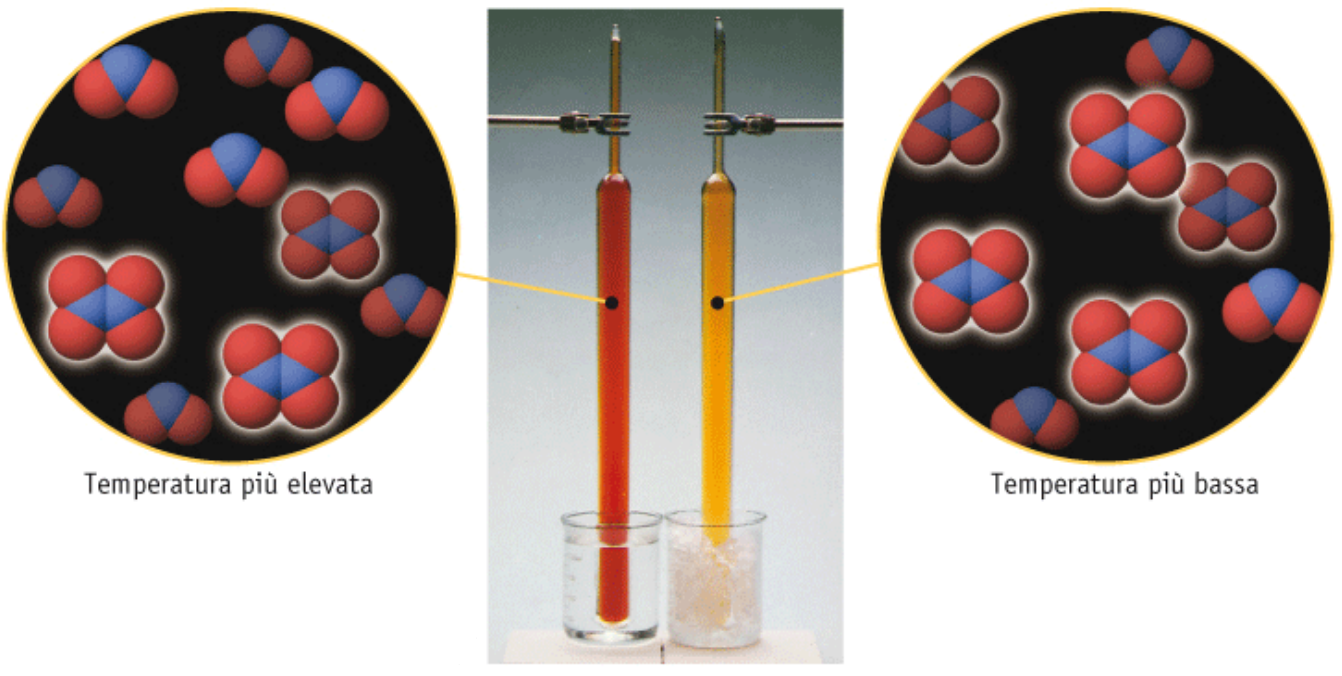
\includegraphics[width=14cm]{immagini/reazione_NO_2.png}
\end{figure}

Nell'immagine sono mostrati due tubi, i quali contengono entrambi NO$_2$ e N$_2$O$_4$ all'equilibrio. Entrambi sono inoltre immersi in un recipiente, solo che quello che a sinistra contiene acqua a 50° C, quello a destra ghiaccio.

$k_c$ è più grande a temperatura più bassa, poiché l'equilibrio favorisce la produzione di N$_2$O$_4$ incolore. Ciò si osserva chiaramente nel tubo di destra, dove il contenuto è solo leggermente colorato, fatto che indica una bassa concentrazione del gas NO$_2$. A destra invece, dove la temperatura è maggiore, l'equilibrio è spostato verso NO$_2$, come è indicato dall'intensa colorazione marrone.

\vspace{0.2cm}Va poi da notare che se siamo in una reazione di equilibrio non scompariranno mai i reagenti, perché se scomparissero per dare solo prodotti non sarebbe più un equilibrio:

\begin{figure}[H]
    \centering
    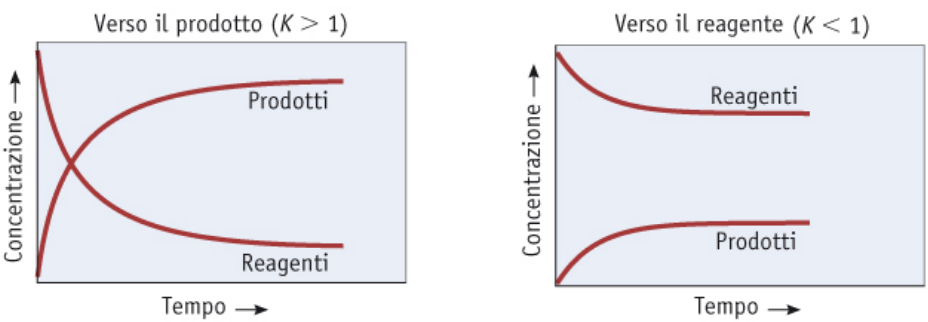
\includegraphics[width=15cm]{immagini/reazioni_equilibrio_spostato.png}
\end{figure}

Nel primo grafico abbiamo una certa concentrazione iniziale di reagenti che diminuisce fino a diventare costante quando viene raggiunto l'equilibrio mentre i prodotti inizialmente non esistevano, ma poi iniziano a formarsi fino a raggiungere una concentrazione costante all'equilibrio. Notiamo che la concentrazione finale dei reagenti è bassa, quella dei prodotti è alta. Possiamo allora dire che questa reazione è spostata verso destra, ossia verso i prodotti. Allora, per come è definita $k_c$, questa sarà maggiore di 1.

Se invece, come nel caso del secondo grafico, la concentrazione dei reagenti diminuisce ma resta lo stesso alta e i prodotti si formano poco cioè hanno una bassa concentrazione, all'equilibrio i reagenti saranno più presenti dei prodotti. Allora, sempre per la definizione di $k_c$, essa sarà minore di 1, ovvero la reazione è spostata verso sinistra, cioè forma poco prodotto: i reagenti restano largamente non reagiti.

\vspace{0.2cm}Quindi il valore di $k_c$ è indicativo di quanto la reazione procede verso destra.

Ad esempio il solfato di bario BaSO$_4$ ha una costante pari a $1.08 \cdot 10^{-10}$, cioè non si scioglie quasi per niente. Ecco perché si può bere.

Quindi l'equilibrio chimico può essere modificato cambiando le concentrazioni, la temperatura o la pressione:
\vspace{0.2cm}\begin{center}
\scriptsize\begin{tabular}{|l|l|l|l|}
    \hline
    & \textbf{Cambiamento quando la} &  &\\
    \textbf{Perturbazione} & \textbf{miscela torna all'equilibrio} & \textbf{Effetto sull'equilibrio} & \textbf{Effetto su $k$}\\
    \hline
    \textit{Reazioni coinvolgenti solidi,}&&&\\
    \textit{liquidi o gas} &&&\\[0.5ex]
    \hline
    Aumento della temperatura & Energia termica è consumata & Spostamento nella dire- & Cambiamento\\
    & dal sistema & zione endotermica &\\[0.5ex]
    \hline
    Diminuzione della & Energia termica è generata & Spostamento nella dire- & Cambiamento\\
    temperatura & dal sistema & zione esotermica &\\
    \hline
    Addizione di un reagente & Il reagente addizionato viene & Aumenta la concen- & Nessun\\
    & in parte consumato & trazione dei prodotti & cambiamento\\[0.5ex]
    \hline
    Addizione di un prodotto & Il prodotto addizionato viene & Aumenta la concen- & Nessun\\
    & in parte consumato & trazione dei reagenti & cambiamento\\[0.5ex]
    \hline
    \textit{Reazioni coinvolgenti gas} &&&\\[0.5ex]
    \hline
    Diminuzione del volume, & Diminuzione della pressione & La composizione cambia & Nessun\\
    diminuzione della pressione & & per ridurre il numero &cambiamento\\
    &&totale delle molecole&\\
    &&gassose&\\[0.5ex]
    \hline
    Aumento del volume, & Aumento della pressione & La composizione cambia & Nessun\\
    diminuzione della pressione & & per ridurre il numero &cambiamento\\
    &&totale delle molecole&\\
    &&gassose&\\
    \hline
\end{tabular}
\end{center}

\vspace{0.2cm}\normalsize La definizione della costante di equilibrio si ottiene però fissando la temperatura. La pressione invece non fa variare il valore della costante, ma ci permette, qualora avessimo variazione del numero di moli, di modificare le concentrazioni finali all'equilibrio.

La temperatura quindi modifica l'equilibrio. Tuttavia può essere necessario cambiarla qualora avessimo una reazione che sia un processo endotermico o esotermico. Se è un processo endotermico, che assorbe calore, riscaldare significherà favorirlo e quindi ottenere più prodotto; se è un processo esotermico, che sviluppa calore, per ottenere più prodotto conviene sottrarre calore.
\subsection{Produzione dell'ammoniaca}
Il progresso industriale di una nazione si misura in rapporto al numero di tonnellate di acido solforico e ammoniaca che produce in un anno.

In particolare l'ammoniaca viene prodotto attraverso il \textbf{processo di Haber-Bosch}.

\vspace{-1cm}\begin{figure}[htp]
    \centering
    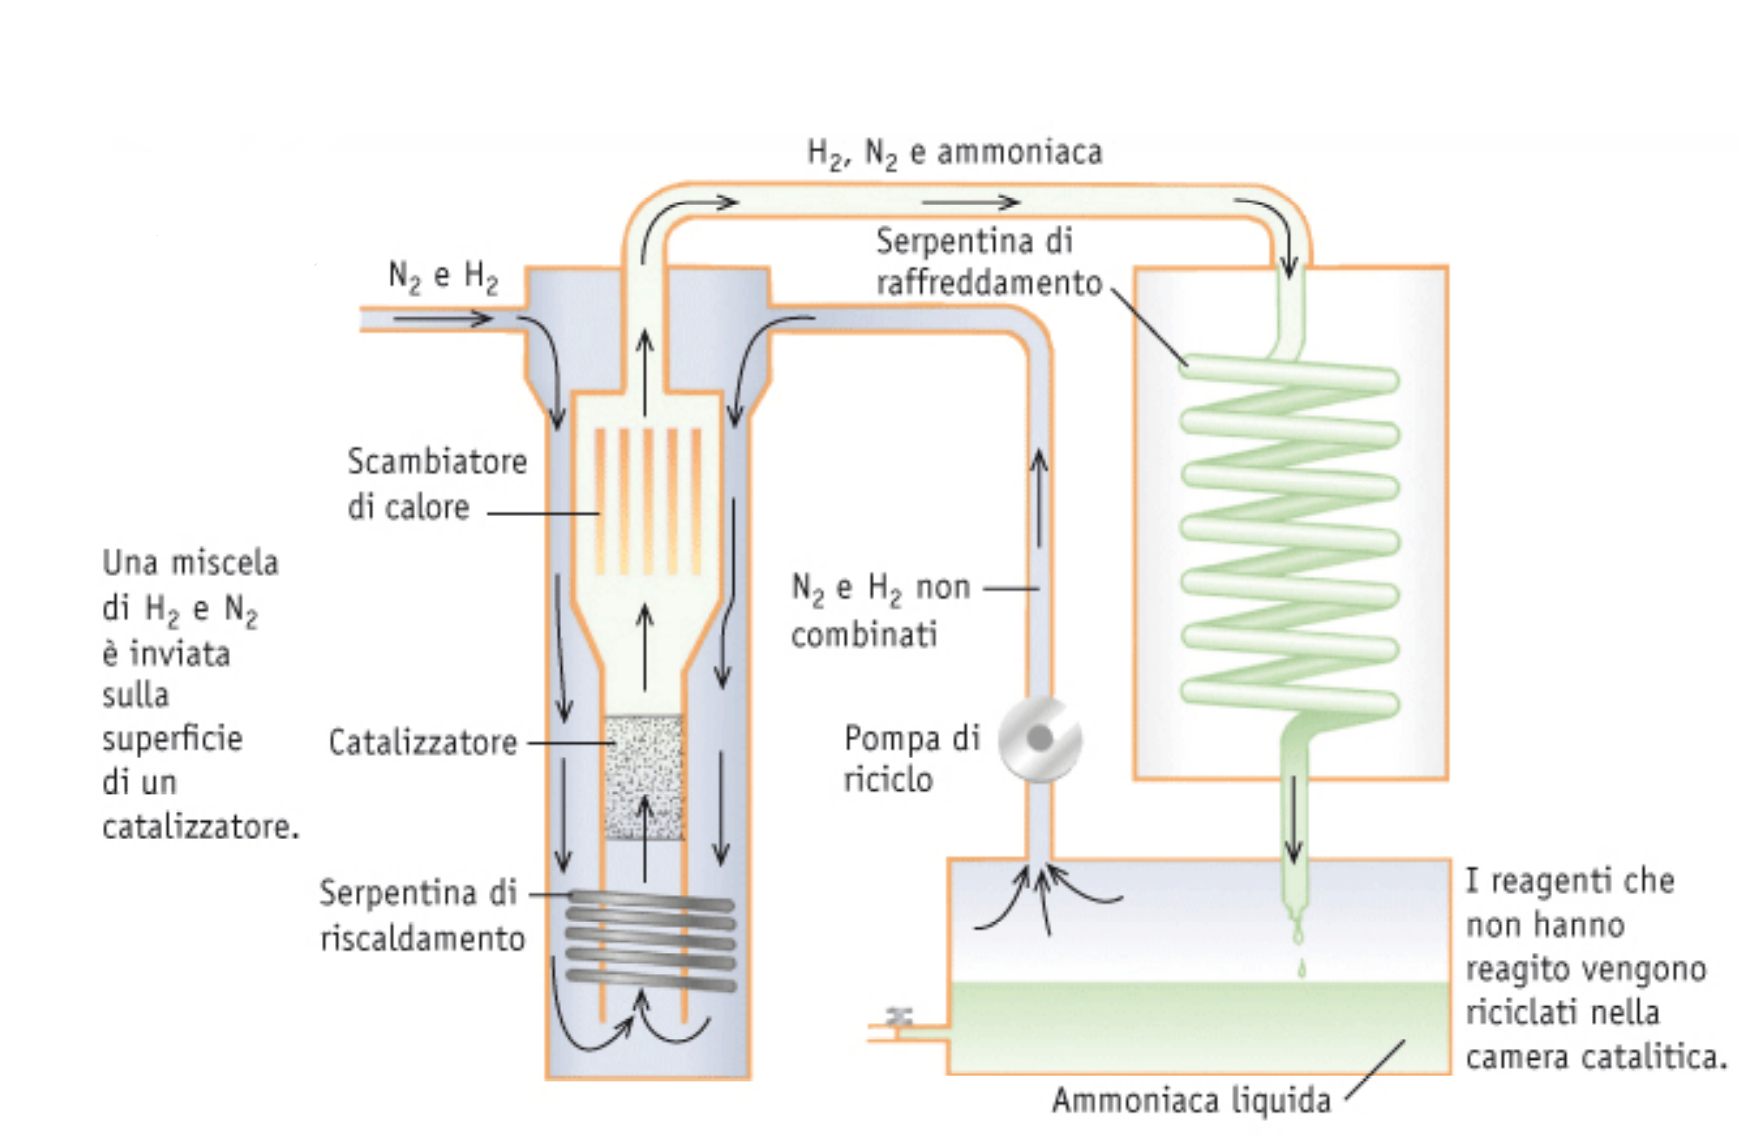
\includegraphics[width=14cm]{immagini/produzione_ammoniaca.png}
\end{figure}

In esso si parte da idrogeno ed azoto gassosi:

$$\ce{N_2(g) + 3H_2(g) <--> 2NH_3(g)}$$

Per avvenire da sola tale reazione, necessita temperature di circa 1000° C. Nella pratica però è possibile abbassare la temperatura a circa 400° C introducendo azoto e idrogeno in un sistema dotato di una serpentina che li riscalda e vengono fatti passare attraverso un catalizzatore che è l'$\rm F_3O_4$ il quale, come si dice in gergo tecnico, permette di abbassare l'energia di attivazione della reazione. Si ottiene così dell'ammoniaca che va condensata a -33° C.

Tuttavia questa è una reazione di equilibrio, quindi parte dei reagenti resteranno non reagiti. Ci sarà allora una pompa che riaspira i gas non reagiti per rinviarli nel sistema e far ripartire il processo.
\newpage
\subsubsection{Valori vari della costante di equilibrio}

Riportiamo adesso alcuni esempi dei valori delle costanti di equilibrio.

\vspace{0.5cm}\hspace{-0.5cm}\scriptsize\begin{tabular}{p{3.4cm}p{1.6cm}p{2.5cm}p{3.4cm}p{1.6cm}p{2.5cm}}
    \textbf{Composto} & \textbf{Formula} & $\boldsymbol{K_{ps}}$ & \textbf{Composto} & \textbf{Formula} & $\boldsymbol{K_{ps}}$\\[0.7ex]
    Perclorato di potassio & KClO$_4$ & $1.05 \cdot 10^{-2}$ & Bromuro di magnesio & AgBr & $7.7 \cdot 10^{-13}$\\[0.7ex]
    Fluoruro di litio & LiF & $1.84 \cdot 10^{-2}$ & Idrossido di zinco & Zn(OH)$_2$ & $1.8 \cdot 10^{-14}$ (a 20° C)\\[0.7ex]
    Carbonato di litio & Li$_2$CO$_3$ & $1.7 \cdot 10^{-3}$ & Carbonato di piombo & PbCO$_3$ & $3.3 \cdot 10^{-14}$ (a 18° C)\\[0.7ex]
    Nitrato di argento & AgNO$_3$ & $5.86 \cdot 10^{-4}$ & Idrossido di manganese & Mn(OH)$_2$ & $4 \cdot 10^{-14}$ (a 18° C)\\[0.7ex]
    Bromato di bario & Ba(BrO$_3$)$_2$ & $2.43 \cdot 10^{-4}$ & Idrossido ferroso & Fe(OH)$_2$ & $1 \cdot 10^{-15}$ \\[0.7ex]
    Solfato di calcio & CaSO$_4$ & $4.93 \cdot 10^{-5}$ & Clpruro di Mercurio & HgCl$_2$ & $2.6 \cdot 10^{-15}$\\[0.7ex]
    Carbonato di magnesio & MgCO$_3$ & $2.6 \cdot 10^{-5}$ (a 12° C) & Idrossido di piombo & Pb(OH)$_2$ & $1 \cdot 10^{-16}$\\[0.7ex]
    Cloruro di piombo & PbCl$_2$ & $1.7 \cdot 10^{-5}$ & Ioduro di argento & AgI & $1.5 \cdot 10^{-16}$\\[0.7ex]
    Solfato di argneto & Ag$_2$SO$_4$ & $1.2 \cdot 10^{-5}$ & Idrossido di cromo (II) & Cr(OH)$_2$ & $2 \cdot 10^{-16}$ \\[0.7ex]
    Idrossido di calcio & Ca(OH)$_2$ & $5.02 \cdot 10^{-6}$ & Idrossido di nichel & Ni(OH)$_2$ & $5.48 \cdot 10^{-16}$ \\[0.7ex]
    Bicromato di argento & Ag$_2$Cr$_2$O$_7$ & $2 \cdot 10^{-7}$ & Solfuro ferroso & FeS & $3.7 \cdot 10^{-19}$ (a 18° C)\\[0.7ex]
    Iodato di rame & Cu(IO$_3$)$_2$ & $1.4 \cdot 10^{-7}$ & Idrossido di rame (II) & $\rm Cu(OH)_2$ & $4.8 \cdot 1o^{-20}$\\[0.7ex]
    Carbonato di calcio & CaCO$_3$ & $0.87 \cdot 10^{-8}$ & Bromuro di mercurio & HgBr$_2$ & $8 \cdot 10^{-20}$\\[0.7ex]
    Solfato di piombo & PbSO$_4$ & $1.06 \cdot 10^{-8}$ (a 18° C) & Fosfato di alluminio & AlPO$_4$ & $9.84 \cdot 10^{-21}$\\[0.7ex]
    Ioduro di piombo & PbI$_2$ & $1.39 \cdot 10^{-8}$ & Solfuro di manganese & MnS & $10^{-22}$\\[0.7ex]
    Idrossido di argento & AgOH & $1.52 \cdot 10^{-8}$ (a 20° C)& Idrossido di berillio & Be(OH)$_2$ & $6.92 \cdot 10^{-22}$\\[0.7ex]
    Fluoruro di piombo & PbF$_2$ & $3.2 \cdot 10^{-8}$ & Solfuro di zinco & ZnS & $1.2 \cdot 10^{-23}$ (a 18° C)\\[0.7ex]
    Fluoruro di magnesio & MgF$_2$ & $6.4 \cdot 10^{-9}$ & Idrossido stannoso & Sn(OH)$_2$ & $5.45 \cdot 10^{-27}$\\[0.7ex]
    Carbonato di bario & BaCO$_3$ & $8.1 \cdot 10^{-9}$ &Solfuro di stagno (II)  & SnS & $1 \cdot 10^{-28}$\\[0.7ex]
    Carbonato rameico & CuCO$_3$ & $1 \cdot 10^{-10}$ & Solfuro di piombo & PbS & $3.4 \cdot 10^{-28}$ (a 18° C)\\[0.7ex]
    Solfato di bario & BaSO$_4$ & $1.08 \cdot 10^{-10}$ & Ioduro di mercurio & HgI$_2$ & $3.2 \cdot 10^{-29}$ \\[0.7ex]
    Cloruro di argento & AgCl & $1.56 \cdot 10^{-10}$ & Idrossido di cromo (III) & Cr(OH)$_3$ & $6.3 \cdot 10^{-31}$\\[0.7ex]
    Idrossido di magnesio & Mg(OH)$_2$ & $1.2 \cdot 10^{-11}$ (a 18° C) & Idrossido di alluminio & Al(OH)$_3$ & $3 \cdot 10^{-34}$\\[0.7ex]
    Fluoruro di calcio & CaF$_2$ & $3.95 \cdot 10^{-11}$ & Solfuro rameoso & Cu$_2$S & $2 \cdot 10^{-47}$ (a 18° C)\\[0.7ex]
    Carbonato di manganese & MnCO$_3$ & $9 \cdot 10^{-11}$ & Solfuro di argento & Ag$_2$S & $1.6 \cdot 10^{-49}$ (a 18° C)\\[0.7ex]
    Carbonato di argento & Ag$_2$CO$_3$ & $6.15 \cdot 10^{-12}$ & Solfuro di mercurio & HgS & $1 \cdot 10^{-50}$ (a 18° C)\\[0.7ex]

\end{tabular}

\vspace{0.4cm}

\footnotesize\begin{tabular}{p{9.5cm}p{2.3cm}p{3.3cm}}
    & Costante di & Reazione spostata\\
    & equilibrio, $k$ & verso i prodotti o i\\
        Reazione & (a 25° C) & reagenti all'equilibrio\\
        \hline
        Reazione di combinazione di non metalli&&\\[0.5ex]
        \ce{S(s) + O_2(g) <--> SO_2(g)} & $4.2 \cdot 10^{52}$ & $k>1$; prodotti\\[0.7ex]
        \ce{2H_2(g) + O_2(g) <--> 2H_2O(g)} & $3.2 \cdot 10^{81}$ & $k>1$; prodotti\\[0.7ex]
        \ce{N_2(g) + 3H_2(g) <--> 2NH_3(g)} & $3.5 \cdot 10^8$ & $k>1$; prodotti\\[0.7ex]
        Reazioni di ionizzazione di acidi e basi deboli &&\\[0.5ex]
        \ce{HCO_2H(aq) + H_2O($l$) <--> HCO_2^-(aq) + H_3O^+} & $1.8 \cdot 10^{-4}$ & $k<1$; reagenti\\
        acido formico &&\\[0.7ex]
        \ce{CH_3CO_2(aq) + H_2O($l$) <--> CH_3CO_2^-(aq) + H_3O^+(aq)} & $1.8 \cdot 10^{-5}$ & $k<1$; reagenti\\
        acido acetico&&\\[0.7ex]
        \ce{H_2CO_3(aq) + H_2O($l$) <--> HCO_3^-(aq) + H_3O^+(aq)} & $4.2 \cdot 10^{-7}$ & $k<1$; reagenti\\
        acido carbonico&&\\[0.7ex]
        \ce{NH_3(aq) + H_2O($l$)} & $1.8 \cdot 10^{-5}$ & $k<1$; reagenti\\
        ammoniaca&&\\[0.7ex]
        Reazione di dissoluzione di solidi "insolubili"&&\\[0.7ex]
        \ce{CaCO_3(s) <--> Ca^{2+}(aq) + CO_3^{2-}(aq)} & $3.8 \cdot 10^{-9}$ & $k<1$; reagenti\\[0.7ex]
        \ce{AgCl(s) <--> Ag^+(aq) + Cl^-(aq)} & $1.8 \cdot 10^{-10}$ & $k<1$; reagenti\\[0.7ex]
\end{tabular}